\section{Resultados}
    \subsection{Código}
        \begin{lstlisting}
        1;

        function v = f(v_3)
            mu = 36
            v_s = 1

            if abs(v_3) < v_s
                v = mu * v_3
            elseif v_3 > v_s
                v = mu * v_s
            elseif v_3 < -v_s
                v = -mu * v_s
            endif
        endfunction

        function xdot = df(v, t)
            xdot = zeros (3,1)
            
            xdot(1) = -f(v(3)) - 2*v(1) + v(2)
            xdot(2) = v(1) - 2*v(2) + v(3)
            xdot(3) = v(2) - v(3)
        endfunction
        
        t = linspace (0, 20, 1000); # [0, 20], 1000 steps

        y_1 = lsode("df", [0, 5, 0], t) # v_2(0) = 5
        y_2 = lsode("df", [0, 15, 0], t) # v_2(0) = 15

        plot(t, y_1(:,2), t, y_2(:,2))
        xlabel("t[s]")
        ylabel("v[V]")
        \end{lstlisting}

    \subsection{Gráfico de $v_2$}
        \begin{figure} [H] 
            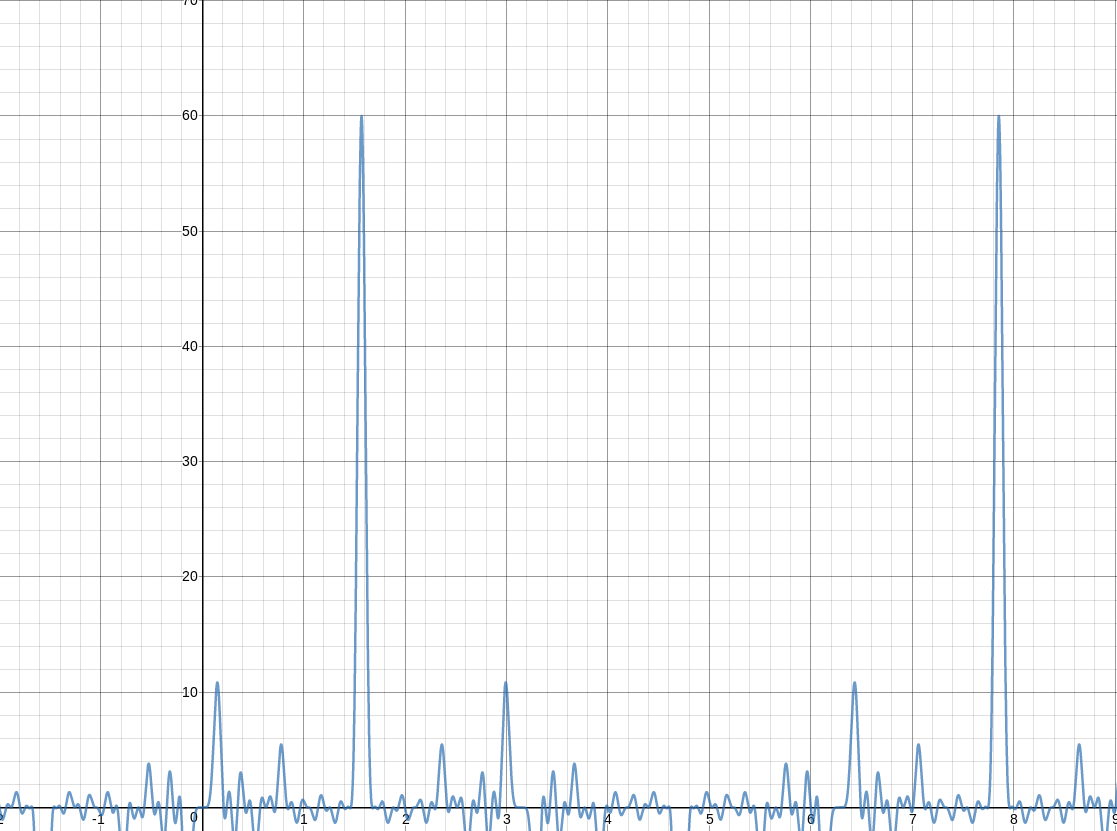
\includegraphics[width=\textwidth]{graph}
            \caption{Gráfico do de $v_2(t)$}
            \label{fig:fraphV2}
        \end{figure}